\begin{figure}[h]
\centering
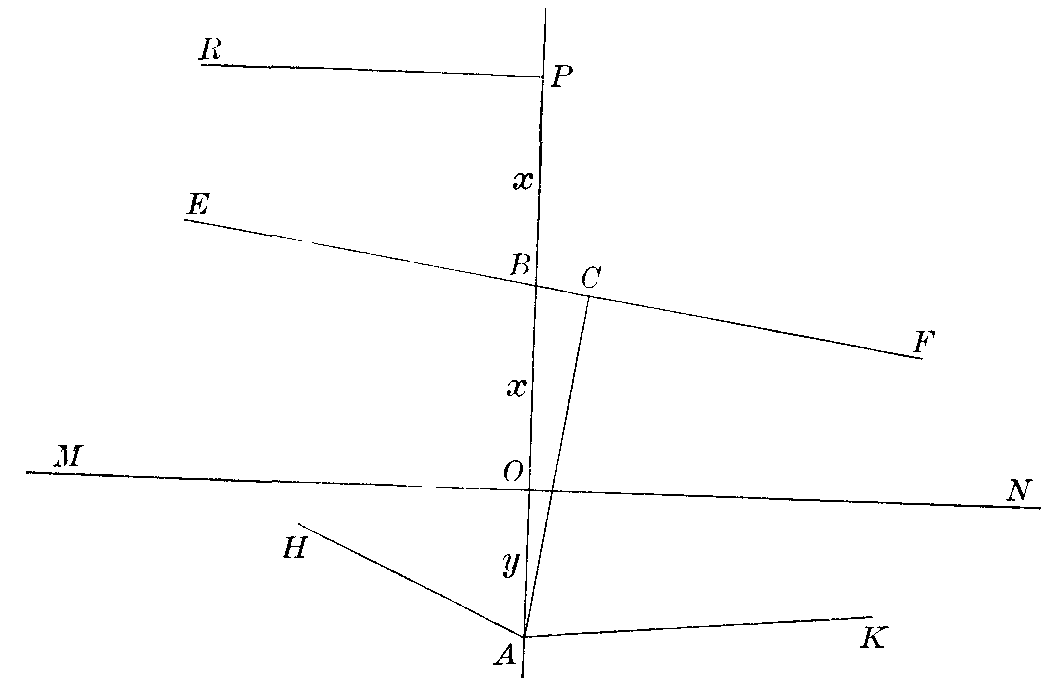
\includegraphics[width=80mm]{fig57.png}
\end{figure}

\item[3.~] 与えられた直線 $MN$ の点 $O$ に垂線を立て、この垂線上に、$MN$ の下側に $OA = y$ をとり、$MN$ の上側に $OB$ と $BP$ をそれぞれ $x$ にとる。$x$ と $y$ は任意の長さとする。$P$ で $OP$ に垂直に、左へ延びる $PR$ を引き、$B$ を通って、$OP$ と角 $\Pi (x)$ をなす $EF$ を引く。これは一方では $ON$ に、他方では $PR$ に平行である。最後に、$A$ を通る $EF$ への二本の平行線 $AK$ と $AH$ を引く。

点 $A$ には四つの平行角がある。
\begin{align*}
 CAK = CAH &= \Pi (AC),       \\
       OAK &= \Pi (y) ,       \\
       PAH &= \Pi (y+2x) .    \\
\intertext{したがって、}
   \Pi (y) &= \Pi (AC) + BAC ,\\
\intertext{および}
\Pi (y+2x) &= \Pi (AC) - BAC . \\
\intertext{さて直角三角形 $ABC$ において}
\cos \Pi (y + x) &= \frac{\cos \Pi (AC)}{\cos BAC} \\
\intertext{すなわち}
  \frac{1-\cos \Pi (y+x)}{1+\cos \Pi (y+x)}
&= \frac{\cos BAC - \cos \Pi (AC)}{\cos BAC + \cos \Pi (AC)}, \\
&= \frac{ \sin \tfrac{1}{2} \left[ \Pi (AC) + BAC \right]
          \sin \tfrac{1}{2} \left[ \Pi (AC) - BAC \right] }
        { \cos \tfrac{1}{2} \left[ \Pi (AC) + BAC \right]
          \cos \tfrac{1}{2} \left[ \Pi (AC) - BAC \right] }; \\
\intertext{ゆえに、}
\tan^2 \tfrac{1}{2} \Pi (y + x)
  &= \tan \tfrac{1}{2} \Pi (y) \tan \tfrac{1}{2} \Pi (y + 2x)
\end{align*}

そこで $\tan \frac{1}{2} \Pi(x)$ は $x$ の関数、たとえば $f(x)$ であって、条件
\begin{align*}
  \left[ f(y + x) \right]^2 & = f(y) f(y+2x) \\
\intertext{すなわち}
  \frac{f(y+x)}{f(y)} & = \frac{f(y+2x)}{f(y+x)}
\end{align*}
を満たす。この式の $y$ に $y + x$、$y + 2x$、$\cdots$ を順次代入してゆくと、さらに
\begin{equation*}
= \frac{f(y+3x)}{f(y+2x)} = \cdots
= \frac{f(y+nx)}{f \left[ y+(n-1)x \right]}
\end{equation*}
を加えることができる。

$\Pi (0) = \frac{\pi}{2}$ で $\tan \tfrac{1}{2} \Pi (0) = 1$ であるから、これらすべての分数の最初と最後に $y = 0$ を代入すると、
\begin{align*}
  f(x) & = \frac{f(nx)}{f\left[ (n-1) x\right]} , \\
\intertext{すなわち}
  f(nx) & = f\left[(n-1)x \right] f(x). \\
\therefore f(nx) & = \left[ f(x)\right]^n
\end{align*}
を得る。

この式は指数関数に特有のものである。\footnote{前出の脚注を見よ。} $\Pi (x)$ は鋭角であるから $\tan \tfrac{1}{2} \Pi (x) < 1$ であり、したがって $f(1) = e^{-a'}$ と書けて、$f(x) = e^{-a'x}$ となる。$a'$ は測定の単位に依存する。ここでは $a' = 1$ となるように単位をとる。最後に、$\Pi(-x) = \pi - \Pi (x)$ であるから、
\begin{equation*}
\tan \tfrac{1}{2} \Pi (-x)
  = \cot \tfrac{1}{2} \Pi (x)
  = \left[ \tan \tfrac{1}{2} \Pi (x) \right]^{-1}
\end{equation*}
である。
\newpage
すなわち、$x$ のすべての実数値に対して、
\begin{align*}
    \tan \tfrac{1}{2} \Pi (x) &= e^{-x} ,
\intertext{すなわち}
\frac{1-\cos\Pi(x)}{\sin\Pi(x)}
  &= \cos ix + i\sin ix.\footnotemark
\end{align*}
\footnotetext{$i$ は $\sqrt{-1}$ を表す。指数関数と三角関数の関係を得る最良の方法は、それらの級数展開によるものである。
\begin{align*}
  e^x &= 1 + x + \frac{x^2}{2!} + \dots + \frac{x^n}{n!} + \dotsb,\\
  \cos x &= 1 - \frac{x^2}{2!} + \frac{x^4}{4!} - \dots +
           (-1)^n\frac{x^{2n}}{2n!} + \dotsb,\\
  \sin x &= x - \frac{x^3}{3!} + \frac{x^5}{5!} - \dots +
           (-1)^n\frac{x^{2n+1}}{(2n+1)!} + \dotsb.
\end{align*}
\par これらの級数は $x$ のすべての値に対して収束する。
\par $x$ に $ix$ を代入すると、
\begin{gather*}
  \begin{aligned}
    e^{ix} &= 1 + ix - \frac{x^2}{2!} - \frac{ix^3}{3!} + \dotsb\\
    &= 1 - \frac{x^2}{2!} + \frac{x^4}{4!} - \dots +
    i\left( x - \frac{x^3}{3!} + \frac{x^5}{5!} - \dotsb \right);
  \end{aligned} \\
  \begin{aligned}
\text{すなわち}\qquad e^{ix}  &= \cos x + i\sin x.\\
\text{また}\qquad e^{-ix} &= \cos x - i\sin x.\\
    \therefore \cos x &= \tfrac{1}{2} \left(e^{ix} + e^{-ix}\right),\\
    \sin x &= \tfrac{1}{2i} \left(e^{ix} - e^{-ix}\right).
  \end{aligned}
\end{gather*}
\par さらに、$x$ に $ix$ を代入すると、
\begin{align*}
  e^x &= \cos ix - i\sin ix,\\
  e^{-x} &= \cos ix + i\sin ix;\\
  \intertext{および}
  \cos ix &= \tfrac{1}{2} \left(e^x + e^{-x}\right),\\
  \sin ix &= -\tfrac{1}{2i} \left(e^x - e^{-x}\right).\\
  \cos ix &= 1 + \frac{x^2}{2!} + \frac{x^4}{4!} + \dotsb,\\
  \sin ix &= ix \left(1 + \frac{x^2}{3!} + \frac{x^4}{5!}
                                                     + \dotsb\right).
\end{align*}
\par $x$ の実数値に対して、$\cos ix$ と $\dfrac{\sin ix}{ix}$ は実数で正であり、$x$ が $0$ から $\infty$ まで変化するとき、$1$ から $\infty$ まで変化する。
\par 等式 $\cos^2ix + \sin^2ix = 1$ において、第一項は $x$ の実数値に対して実数で正であり、第二項は実数で負である。したがって、$\sin ix$ は絶対値において $\cos ix$ より小さく、$\tan ix$ は絶対値において $1$ より小さい。$\tan ix$ は、$x$ が $0$ から $\infty$ まで変化するとき、絶対値において $0$ から $1$ まで変化する。}

$x$ の符号を変えると、
\begin{align*}
\frac{1+\cos\Pi(x)}{\sin\Pi(x)} &= \cos ix - i \sin ix, \\
\intertext{加えたり引いたりして、}
\frac{1}{\sin\Pi(x)} &= \cos ix, \\
\cot\Pi(x) &= -i\sin ix
\end{align*}
を得る。

したがって、平行角の性質は、方程式
\begin{align*}
\sin\Pi(x) &= \frac{1}{\cos ix}, \\
\tan\Pi(x) &= \frac{i}{\sin ix}, \\
\cos\Pi(x) &= \frac{\tan ix}{i}
\end{align*}
で表される。

\item[4.~] 平面直角三角形の公式に代入すると、それらは、$a$、$b$、$c$ の代わりにそれぞれ $ia$、$ib$、$ic$ を用いた球面直角三角形の公式に帰着することがわかる。斜角三角形の公式は、球面上と同じ方法で直角三角形の公式から得られ、こうして、平面三角法のすべての公式が、球面三角法の公式からこの変更をするだけで得られる。

斜角三角形の基本公式として、次を書く。
\begin{gather*}
\frac{\sin A}{\sin ia} = \frac{\sin B}{\sin ib}
                       = \frac{\sin C}{\sin ic}, \\
\cos ia = \cos ib\, \cos ic + \sin ib\, \sin ic\, \cos A, \\
\cos A  = -\cos B\, \cos C + \sin B\, \sin C\, \cos ia.
\end{gather*}

$\Pi$ 関数の記法では、これらは次のようになる。
\begin{gather*}
\sin A\, \tan\Pi(a) = \sin B\, \tan\Pi(b) = \sin C\, \tan\Pi(c), \\
\frac{\sin\Pi(b)\,\sin\Pi(c)}{\sin\Pi(a)} =
                             1-\cos\Pi(b)\,\cos\Pi(c)\,\cos A, \\
\cos A = -\cos B\, \cos C + \frac{\sin B\,\sin C}{\sin\Pi(a)}.
\end{gather*}

\item[5.~] $x$ が非常に小さい値のとき、近似的に
\begin{gather*}
\sin ix = ix, \\
\cos ix = 1 + \frac{x^2}{2}, \\
\tan ix = ix, \\
\intertext{であるから、無限小の三角形についての公式は次に帰着する。}
\frac{\sin A}{a} = \frac{\sin B}{b} = \frac{\sin C}{c}, \\
a^2 = b^2 + c^2 - 2bc\,\cos A, \\
\cos A = -\cos(B+C).
\end{gather*}

\item[6.~] 等距離面上の三角形は、基底平面への射影と相似である。すなわち、角が同じで、辺が比例する。したがって、平面三角法の公式は、辺を表す文字に、$i$ のほかに、曲面の平面からの距離に依存する定数因子をつければ、任意の等距離面について成り立つ。
\end{description}
